\chapter{Usabilidade}
\label{cap-usabilidade}

\section{Terminologias}
\label{sec-terminologias}

% No TCC 2, talvez, terminologia deve ser um capítulo inicial do trabalho.

O termo usabilidade de modo geral pode ser escrito como a facilidade com a qual
um equipamento ou programa pode ser usado. Esse termo dentro da computação foi
diversas vezes refinado como nas ISO 9126, 12119, 9241, 14598 e, por fim, na ISO
25010, que define como uma medida pela qual um produto pode ser usado por
usuários específicos para alcançar metas específicas com eficácia, eficiência e
satisfação em um contexto específico de uso~\cite{}.
%TODO: colocar referência da ISO.

%
A usabilidade não é uma qualidade intrínseca de um sistema, é dependente de um
acordo entre as características de sua interface e as características de seus
usuários na busca de determinados objetivos e situação de uso~\cite{}.
%TODO: referência para Cybis, 2010]
%
Por esse motivo uma interface que pode ser considerada satisfatória para
determinado grupo de usuários pode ser inviabilizada por outros, como usuários
experientes \textit{versus} novatos, além de uma percepção diferente dependendo
do ambiente onde esse sistema se encontra, um computador lento \textit{versus}
computador rápido.
%
Dessa forma, podemos definir que a usabilidade é um acordo entre interface,
usuário, tarefa e ambiente. Baseado nesta definição é que pautaremos nossas
discussões e estudos de caso neste trabalho.

%
A necessidade de se garantir que sistemas e dispositivos estejam
adaptados à maneira como o usuário pensa, comporta-se e trabalha, entra o
conceito de ergonomia.
%
Tal conceito surgiu logo após a II Guerra Mundial, como consequência do trabalho
interdisciplinar realizado por diversos profissionais, tais como engenheiros,
fisiologistas e psicólogos, durante a guerra~\cite{}.
%TODO: referenciar Lida, 2005

%
Há algumas definições formais para o termo ``ergonomia'', de acordo com a
\textit{Ergonomics Society}, a Associação Brasileira de Ergonomia e a 
\textit{International Ergonomics Association}.
%
Para este trabalho, adotamos a definição da Associação Brasileira de Ergonomia,
que a conceitua como o estudo das interações das pessoas com a tecnologia, a
organização e o ambiente, objetivando intervenções e projetos que visem
melhorar, de forma integrada e não-dissociada, a segurança, o conforto, o
bem-estar e a eficácia das atividades humanas \cite{}.
%TODO: referência para o texto da ABE.

%
Neste contexto, a questão que norteia este trabalho é como pode-se avaliar,
entender, verificar, observar a interface de uma aplicação em determinado
contexto ou sistema?
%
Para respondermos essa questão, mapeamos as definições de alguns especialistas
em usabilidade e ergonomia, que estabeleceram critérios, regras e princípios
para nortear essa necessidade.

\begin{itemize}
\item Jakob Nielsen, em seu livro \textit{Usability Engineering} , propõe um
conjunto de dez heurísticas de usabilidade~\cite{}:
%TODO: referência para o livro Usability Engineering

    \begin{itemize} 

    \item Viabilidade do estado do sistema;

    \item Mapeamento entre o sistema e o mundo realizada;

    \item Liberdade e controle ao usuário;

    \item Consistência e padrões;

    \item Prevenção de erros;

    \item Reconhecer em vez de relembrar;

    \item Flexibilidade e eficiência de uso;

    \item Design estético e minimalista;

    \item Suporte para o usuário reconhecer, diagnosticar e recuperar erros;

    \item Ajuda e documentação.

    \end{itemize}

\item Ben Shneiderman, em seu  \textit{livro Designing The User Interface},
propõe, o que ele denominou de ``oito regras de ouro'':

    \begin{itemize} 

    \item Perseguir a consistência;

    \item Fornecer atalhos;

    \item Fornecer feedback informativos;

    \item Marcar o final dos diálogos;

    \item Fornecer prevenção e manipulação simples de erros;

    \item Permitir o cancelamento das ações;

    \item Fornecer controle e iniciativa ao usuário;

    \item Reduzir a carga de memória de trabalho.

    \end{itemize}

\item Christian Bastien e Dominique Scapin definiram 8 critérios ergonômicos:
%TODO: completar (Primeiro e segundo nome dos autores para ficar igual aos
%      anteriores) e colocar as referências

    \begin{itemize}

    \item Condução;

    \item Carga de trabalho;

    \item Controle;

    \item Adaptabilidade;

    \item Gestão de erros;

    \item Coerência;

    \item Significado dos códigos;

    \item Denominações e Compatibilidade.

    \end{itemize}

\end{itemize}

Portanto, baseado nas heurísticas e critérios listados acima,  Walter Cybis, no
livro Ergonomia e Usabilidade, propôs uma tabela que relaciona todas essas
definições, conforme aprensentado na Tabela \ref{tabela-walter-cybis}~\cite{}.
%TODO: referência de  Walter Cybis
\begin{table}[h]
\begin{tabular}{|l|l|}
\hline
Condução                               & \begin{tabular}[c]{@{}c@{}}Qualidade da ajuda e da documentação\\ Adequação ao aprendizado\\ Apresentação do estado do sistema\\ Convite\\ Agrupamento e distinção por localização\\ Agrupamento e distinção por formato\\ Feedback imediato\end{tabular} \\ \hline
Carga de trabalho                      & \begin{tabular}[c]{@{}c@{}}Legibilidade\\ Brevidade das entradas individuais\\ Concisão das apresentações individuais\\ Ações mínimas\\ Densidade informacional\\ Design minimalista e estético\end{tabular}                                              \\ \hline
Controle                               & \begin{tabular}[c]{@{}c@{}}Ações explícitas\\ Controle do usuário\end{tabular}                                                                                                                                                                            \\ \hline
Adaptabilidade                         & \begin{tabular}[c]{@{}c@{}}Flexibilidade\\ Personalização\\ Consideração da experiência do usuário\end{tabular}                                                                                                                                           \\ \hline
Gestão de erros                        & \begin{tabular}[c]{@{}c@{}}Proteção de erros\\ Tolerância aos erros\\ Qualidade das mensagens de erro\\ Correção de erros\end{tabular}                                                                                                                    \\ \hline
Coerência                              & \begin{tabular}[c]{@{}c@{}}Homogeneidade interna a uma aplicação\\ Homogeneidade externa a plataforma\end{tabular}                                                                                                                                        \\ \hline
Significado dos códigos e denominações & Interface clara                                                                                                                                                                                                                                           \\ \hline
Compatibilidade                        & \begin{tabular}[c]{@{}c@{}}Compatibilidade com o usuário\\ Compatibilidade com a tarefa dos usuários\\ Compatibilidade com a cultura dos usuários\end{tabular}                                                                                            \\ \hline
\end{tabular}
\caption{Conjunto integrador de critérios, princípios, regras e heurísticas de ergonomia}	
\label{tabela-walter-cybis}
\end{table}

\section{Técnicas de Usabilidade Ágeis}
\label{técnicas-usabilidade-ageis}


Técnicas de usabilidade e desenvolvimento ágil têm muito em comum, principalmente o fato de que, muitas vezes, estão envolvidos no desenvolvimento do mesmo software. Apesar disso, tem havido pouca investigação ou discussão sobre a forma como os dois processos trabalham em conjunto e os resultados dessa parceria. ~\cite{}.%Jennifer Ferreira 1 , James Noble 1 E Robert Biddle

%
Para tanto realizou-se uma revisão sistemática. A revisão sistemática é uma forma de síntese das informações disponíveis em dado momento, sobre um
problema específico, de forma objetiva e reproduzível, por meio de método científico. Ela tem como princípios gerais a exaustão na busca dos estudos analisados, a seleção justificada dos estudos por critérios de inclusão e exclusão explícitos e a avaliação da qualidade metodológica, bem
como a quantificação do efeito dos tratamentos por meio de técnicas estatísticas.\cite{}%Lima MS de, Soares BGO, Bacaltchuk J. Psiquiatria baseada em evidências. Rev Bras Psiquiatr 2000 setembro; 22(3):142- 6.
O Objetivo da revisão sistemática era levantar as técnicas de usabilidade em projetos ágeis aplicadas no desenvolvimento de software livre. A busca foi realizada nas bibliotecas digitais Google Academic e Springer Link que possuem máquinas de busca com bom funcionamento e abrangência, além das bases de teses e dissertações da UnB e USP. nas Como resultado do trabalho levantou-se uma lista de técnicas e selecionadas aquelas que poderiam ser mais facilmente aplicadas em projetos de software livre.

%
Santos e Kon (2012) propõe a aplicação do próprio processo de DCU (Design Centrado no Usuário) para levantamento dos usuários e do contexto de uso da metodologia. Os usuários do processo são membros de equipes de software livre, que desejam inserir práticas de usabilidade no processo de desenvolvimento. O contexto de uso são sistemas distribuídos geograficamente, com pessoas trabalhando colaborativamente. Os métodos podem ser aplicados tanto para o início de novos projetos, que tenham como usuários, pessoas não acostumadas a sistemas livres ou mesmo para a melhoria de sistemas existentes, com respeito à usabilidade.~\cite{}%Aplicação de metodologias ...

%
Já Lee, Judge e McCrickard (2011) defendem a aplicação de definição de histórias de usuário de usabilidade dirigidas pela decisão do responsável por design realizando a prototipação dessas histórias e depois sendo validadas através de testes de usabilidade conforme Figura \ref{fig:figuraCDR}~\cite{}.

\begin{figure}[H]
  \begin{center}
    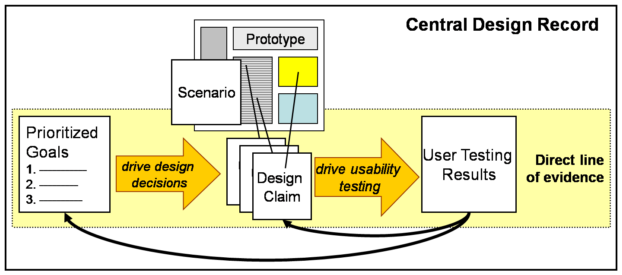
\includegraphics[width=0.5\textwidth]{figuras/figuraCDR.png}
    \caption{Ciclo de atividades de usabilidade}
    \label{fig:figuraCDR}
  \end{center}
\end{figure}

%
As atividades de usabilidade seguem o modelo de ciclo de vida das outras atividades dentro do desenvolvimento ágil com a diferença que o ciclo de usabilidade tem sua iteração primeiro que as outras atividades de desenvolvimento conforme Figura \ref{fig:figuraCDR2}:

\begin{figure}[H]
  \begin{center}
    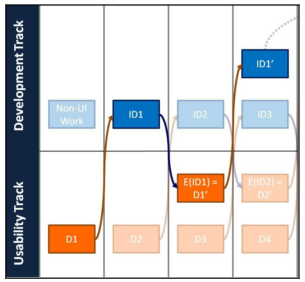
\includegraphics[width=0.5\textwidth]{figuras/figuraCDR2.png}
    \caption{Ciclo das tarefas de usabilidade x desenvolvimento}
    \label{fig:figuraCDR2}
  \end{center}
\end{figure}

%
Santos (2012) em uma nova pesquisa aplicada propós a aplicação das técnicas de usabilidade de acordo com as fases do DCU, conforme a descrição das técnicas de usabilidade das comunidades de métodos ágeis e de software livre. Para a fase do DCU Criar soluções de design, não foram identificadas propostas de adaptações, sendo portanto, descritas propostas para as fases: Identificar necessidades para design centrado em humano, Especificar contexto de uso, Especificar requisitos e Avaliar Designs conforme Figura \ref{fig:figuraDCU}.

\begin{figure}[H]
  \begin{center}
    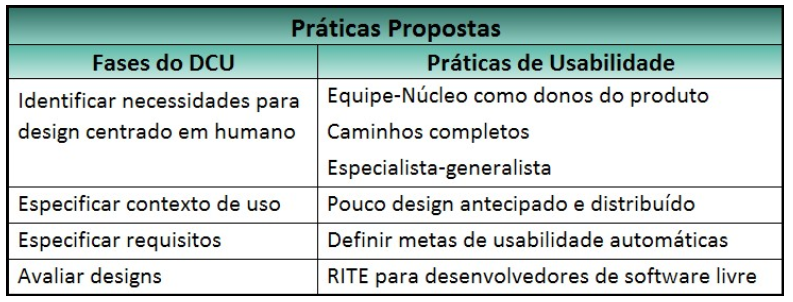
\includegraphics[width=0.7\textwidth]{figuras/figuraDCU.png}
    \caption{Técnicas de usabilidade baseado no DCU}
    \label{fig:figuraDCU}
  \end{center}
\end{figure}

%
Moreno e Yagüe (2012) trás em seu trabalho a inserção da usabilidade por meio da criação de User Stories de usabilidade que denominam de \textit{Usability Stories}. Tendo que especificar os recursos funcionais de usabilidade que serão utilizados no projeto, o artigo trás um tabela que é necessária para definir as características dessa funcionalidade.

\begin{table}[H]
\begin{tabular}{|l|l|}
\hline
Status do Sistema                                                      & Para informar os usuários sobre a situação interna do sistema                                                                                                                                                \\ \hline
Aviso                                                                  & \begin{tabular}[c]{@{}c@{}}Para informar os usuários de qualquer ação com conseqüências\\  importantes\end{tabular}                                                                                          \\ \hline
Longa ação Feedback                                                    & \begin{tabular}[c]{@{}c@{}}Para informar aos usuários que o sistema está processando\\  uma ação que vai demorar algum tempo para completar\end{tabular}            \\ \hline
Desfazer global                                                        & Para desfazer as ações do sistema em vários níveis                                                                                                                                                           \\ \hline
Abortar Operação                                                       & Para cancelar a execução de uma ação ou toda a aplicação                                                                                                                                                     \\ \hline
Abortar comando                                                        & Para cancelar a execução de uma tarefa em andamento                                                                                                                                                          \\ \hline
Voltar                                                                 & \begin{tabular}[c]{@{}c@{}}Para voltar a um estado particular em uma seqüência de \\ execução de comando\end{tabular}                                                                                        \\ \hline
\begin{tabular}[c]{@{}c@{}}Entrada de texto\\ estruturada\end{tabular} & \begin{tabular}[c]{@{}c@{}}Para ajudar a prevenir o usuário de cometer erros de \\ entrada de dados\end{tabular}                                                                                             \\ \hline
\begin{tabular}[c]{@{}c@{}}Execução\\ Passo-a-Passo\end{tabular}       & \begin{tabular}[c]{@{}c@{}}Para ajudar os usuários a realizar tarefas que requerem \\ diferentes passos com a entrada do usuário e tal entrada correta\end{tabular} \\ \hline
Preferências                                                           & \begin{tabular}[c]{@{}c@{}}Para gravar as opções de cada usuário para usar as \\ funções do sistema\end{tabular}                                                                                             \\ \hline
Favoritos                                                              & Para gravar determinados locais de interesse para o usuário                                                                                                                                                  \\ \hline
Ajuda Multinível                                                       & Para fornecer diferentes níveis de ajuda para usuários diferentes                                                                                                                                            \\ \hline
\end{tabular}
\caption{Mecanismos de usabilidade}
\label{tabela-mec-usabilidade}
\end{table}

Associado a essas características é definido três maneiras pelas quais a incorporação de usabilidade influencia as histórias de usuário.
\begin{enumerate}
\item A adição de novas histórias para representar requisitos diretamente derivados usabilidade.
\item Adição ou modificação de tarefas em histórias de usuários existentes. Isto significa que algumas ações decorrentes de limitações de usabilidade devem ser realizadas por um usuário existente na história. Esta tarefa pode ser tão simples ou detalhados, conforme necessário.
\item Adição ou modificação de critérios de aceitação. Estes critérios de aceitação aparecem porque a funcionalidade da história de usuário precisa incluir algumas ações específicas para modificar o ambiente operacional.
\end{enumerate}

Com isso os autores realizaram um mapeamento entre os mecanismos de usabilidade e as ações a serem tomadas finalizando a proposta de como a usabilidade deve ser abordada por equipes ágeis.

\begin{table}[H]
\begin{tabular}{|l|l|l|l|l|l|l|}
\hline
                                                                       & \begin{tabular}[c]{@{}c@{}}Nova\\ Tarefa\end{tabular} & \begin{tabular}[c]{@{}c@{}}Modificar\\ Tarefa\end{tabular} & \begin{tabular}[c]{@{}c@{}}Novo\\ Critério de\\Aceitação\end{tabular} & \begin{tabular}[c]{@{}c@{}}Modificar\\ Critério de\\Aceitação\end{tabular} & \begin{tabular}[c]{@{}c@{}}Nova\\ História de \\ Usabilidade\end{tabular} & \begin{tabular}[c]{@{}c@{}}Nova\\ História\\ de Usuário\end{tabular} \\ \hline
Status do Sistema                                                      &                                                       & X                                                          & X                                                                      & X                                                                           & X                                                                                                                                                           &                                                                      \\ \hline
Aviso                                                                  & X                                                     &                                                            & X                                                                      & X                                                                           & X                                                                                                                                                           &                                                                      \\ \hline
Longa ação                                                             &                                                       & X                                                          & X                                                                      &                                                                             &                                                                                                                                                             & X                                                                    \\ \hline
Abortar Operação                                                       &                                                       & X                                                          & X                                                                      &                                                                             &                                                                                                                                                             &                                                                      \\ \hline
Abortar comando                                                        & X                                                     & X                                                          & X                                                                      &                                                                             &                                                                                                                                                             &                                                                      \\ \hline
Voltar                                                                 & X                                                     & X                                                          & X                                                                      &                                                                             &                                                                                                                                                             &                                                                      \\ \hline
\begin{tabular}[c]{@{}c@{}}Entrada de texto\\ estruturada\end{tabular} &                                                       & X                                                          & X                                                                      &                                                                             &                                                                                                                                                             &                                                                      \\ \hline
\begin{tabular}[c]{@{}c@{}}Execução\\ Passo-a-Passo\end{tabular}       & X                                                     &                                                            & X                                                                      & X                                                                           &                                                                                                                                                             &                                                                      \\ \hline
Preferências                                                           &                                                       &                                                            &                                                                        &                                                                             &                                                                                                                                                             & X                                                                    \\ \hline
Favoritos                                                              &                                                       & X                                                          & X                                                                      &                                                                             & X                                                                                                                                                           &                                                                      \\ \hline
Ajuda Multinível                                                       &                                                       & X                                                          & X                                                                      &                                                                             & X                                                                                                                                                           &                                                                      \\ \hline
\end{tabular}
\caption{Mapeamento entre os mecânismos de usabilidade e ações}
\label{tabela-map}
\end{table}


\section{Usabilidade em Software Livre}
\label{usabilidade-sl}
%
Para aplicação em ambientes distribuídos, abertos e colaborativos, como em comunidades de software livre, implica-se uma adaptação em métodos de usabilidade. Isso ocorre porque em comunidades de desenvolvimento de software livre, não se pode garantir a existência de um indivíduo especialista em usabilidade ou de uma equipe dedicada a essas atividades. A distância física de membros que contribuem com o projeto também dificulta a utilização de métodos de usabilidade que dependem de comunicação face a face. Mesmo assim, a usabilidade deve ainda ser considerada, afinal ela é muito importante para a criação de um sistema de qualidade, em qualquer ambiente.

%
A usabilidade deve fazer parte do desenvolvimento, não apenas em busca de produtos usáveis, mas também de práticas usáveis e de modo a envolver todos os membros de uma equipe considerando o contexto em que as práticas serão aplicadas. Dessa forma, não se tem uma equipe de acordo com os valores de métodos ágeis e de métodos de usabilidade se apenas alguns se preocupam em atender as necessidades dos usuários típicos e clientes, pois todos os membros precisam entender a importância de atendê-las.
~\cite{}
%Citar tese Ana Paula
Ana Paula Oliveira dos Santos, em sua dissertação de mestrado, propôs práticas de usabilidade para a comunidade de software livre através da associação das fases do DCU(Design Centrado no Usuário) com as técnicas de usabilidade da comunidade ágil conforme a tabela \ref{tabela-usabilidade-sl}.

\begin{table}[h]
\begin{tabular}{|l|l|}
\hline
\multicolumn{2}{|c|}{\textbf{Práticas de usabilidade para Software Livre}}                                                                                                                                                                          \\ \hline
\textbf{Fases DCU}                                                                                 & \textbf{Práticas de Usabilidade}                                                                                                 \\ \hline
\begin{tabular}[c]{@{}c@{}}Identificar necessidades para \\ design centrado em humano\end{tabular} & \begin{tabular}[c]{@{}c@{}}Equipe-Núcleo como Donos do Produto\\ Caminhos Completos\\ Especialista-generalista\end{tabular}      \\ \hline
Especificar contexto de uso                                                                        & Pouco design antecipado e distribuído                                                                                            \\ \hline
Especificar Requisitos                                                                             & Definir metas de usabilidade automáticas                                                                                         \\ \hline
Avaliar designs                                                                                    & \begin{tabular}[c]{@{}c@{}}RITE (Rapid Iterative Testing and Evaluation)  \\ para desenvolvedores de software livre\end{tabular} \\ \hline
\end{tabular}
\caption{Práticas de usabilidade no contexto de Software Livre}	
\label{tabela-usabilidade-sl}
\end{table}

As práticas são descritas apresentando um contexto, um problema e uma solução visando a adequação a comunidades de software livre.

\textbf{Identificar necessidades para design centrado em humano}

\textbf{Equipe-Núcleo como Donos do Produto}

Contexto: Equipe de desenvolvimento de software livre composta por desenvolvedores e que não possui especialistas em usabilidade ou UX como membros. Contudo, a equipe-núcleo do projeto percebe a necessidade de compreender melhor os requisitos de negócios e de usabilidade, levando em consideração a visão de clientes e usuários típicos.
Problema: Integrar requisitos de negócio com requisitos de usabilidade em um ambiente que não possui especialistas em usabilidade. Principais forças envolvidas:
\begin{itemize}
\item Força 1: Necessidade de levantamento de requisitos de negócios com clientes e requisitos de usabilidade com usuários típicos, de modo a integrá-los para o desenvolvimento do sistema.
\item Força 2: Não existe garantia de que especialistas em usabilidade ou UX participarão voluntariamente do projeto e/ou não é possível contratá-los. Também não é possível garantir que desenvolvedores voluntários queiram participar dessas atividades.
\end{itemize}
Solução: Uma adaptação da prática Especialistas em UX como Donos do Produto, da comunidade de métodos ágeis, na qual a equipe-núcleo de um projeto de software livre assumiria o papel de Proprietários do Produto, que levam em consideração a usabilidade do sistema. Dessa forma, podem controlar as contribuições para o projeto, com a visão das necessidades de usuários típicos e clientes.

%
\textbf{Caminhos Completos}

Contexto: Equipe de desenvolvimento de software livre composta por desenvolvedores e que não possui especialistas em usabilidade ou UX como membros. Contudo, a equipe-núcleo do projeto precisa empregar práticas de usabilidade durante o desenvolvimento do sistema.
Problema: Realizar práticas de usabilidade em projetos de software livre que não possuem especialistas em usabilidade ou UX. Principais forças envolvidas:
\begin{itemize}
\item Força 1: Necessidade de realizar práticas de usabilidade para pesquisa de usuários, levanta- mento de requisitos e metas de usabilidade, definição de design e avaliações com usuários e clientes.
\item Força 2: Não existe garantia de que especialistas em usabilidade ou UX participarão voluntariamente do projeto e/ou não é possível contratá-los.
\item Força 3: Desenvolvimento distribuído e participação esporádica de membros.
\end{itemize}
Solução: Em vez de caminhos paralelos entre equipe de desenvolvimento e de UX, como ocorre na prática Caminhos paralelos da comunidade de métodos ágeis, a equipe de desenvolvimento executa o ciclo completo de DCU para um conjunto específico de funcionalidades, utilizando-se de Pouco design antecipado ou Pouco design antecipado e distribuído para coletar informações. A prática pode ser executada apenas pela equipe-núcleo do projeto ou mesmo com a participação dos demais contribuidores que desejem participar.

%
\textbf{Especialista-generalista}

Contexto: Equipes de desenvolvimento de software livre, que não possuem especialistas em usabilidade ou UX como membros do time, compostas por desenvolvedores que desejam desenvolver sistemas com melhor usabilidade para usuários típicos.
Problema: Ausência de especialistas em usabilidade ou UX na equipe de desenvolvimento do projeto. Principais forças envolvidas:
\begin{itemize}
\item Força 1: Não existe garantia de que especialistas em usabilidade ou UX participarão voluntariamente do projeto e/ou não é possível contratá-los.
\item Força 2: Desenvolvimento distribuído e participação esporádica de membros.
\end{itemize}
Solução: Os desenvolvedores da equipe-núcleo do projeto aplicam práticas de usabilidade para entender quem são os usuários típicos do sistema, quais são as suas necessidades e em que contexto o sistema seria utilizado, de modo a incluir essas considerações nos requisitos da aplicação. As pesquisas têm baixa granularidade, ou seja, realiza-se apenas o necessário para o entendimento das funcionalidades da próxima iteração. Os requisitos podem ser definidos por meio da escrita de cartões de histórias de usuários, que são validados com o cliente conforme ocorre em comunidades de métodos ágeis. A documentação detalhada dos requisitos pode ser encontrada nos testes de aceitação, que podem ser acessados por qualquer desenvolvedor do sistema, conforme a prática Testes de aceitação de comunidades de métodos ágeis, o que mantém um relatório atualizado das funcionalidades do sistema que atendem ao comportamento esperado. As metas de usabilidade do sistema também podem ser descritas por meio da proposta de prática Definir metas de usabilidade automáticas.


%
\textbf{Especificar contexto de uso}

\textbf{Pouco design antecipado e distribuído}

Contexto: Equipe de desenvolvimento de software livre composta por desenvolvedores e que não possui especialistas em usabilidade ou UX como membros. Membros da equipe-núcleo do projeto e contribuidores encontram-se distribuídos em diversas localidades. Contudo, existe a necessidade de realização de pesquisas presenciais com usuários típicos para melhor compreensão do contexto de uso do sistema.
Problema: Utilizar práticas de usabilidade, em ambiente de desenvolvimento de software livre, para especificar contexto de uso de um sistema, onde membros da equipe estão dispersos em vários locais diferentes. Principais forças envolvidas:
\begin{itemize}
\item Força 1: Distância física entre membros de uma comunidade de desenvolvimento de software livre.
\item Força 2: Necessidade de realização de pesquisas de usabilidade para definição de perfil de usuários típicos e o contexto de uso do sistema.
\item Força 3: Possibilitar a participação de voluntários de diversas culturas.
\end{itemize}
Solução: Equipe-núcleo do projeto é responsável por definir quais são as práticas de usabilidade a serem utilizadas para especificação do contexto de uso de um sistema e também por realizar as práticas presenciais na sua cidade. Membros da equipe, que se encontram dispersos em locais distintos, poderiam aplicar a mesma prática em sua localidade, de modo a obter feedback de usuários com culturas diferentes; por exemplo, replicando testes, sessões de grupos focais ou entrevistas presenciais, em sua região ou país. Desse modo, possibilita-se a obtenção da percepção cultural de vários locais distintos, de modo a explorar o contexto de projetos abertos, no qual podem existir desenvolvedores, usuários, membros da equipe-núcleo e contribuidores em diversas localidades.


%
\textbf{Especificar requisitos}

\textbf{Definir metas de usabilidade automáticas}

Contexto: Desenvolvimento aberto, distribuído e colaborativo, onde desenvolvedores podem entrar e sair do projeto durante o processo de desenvolvimento. Também não existe uma equipe de usabilidade trabalhando em conjunto com a equipe de desenvolvimento.
Problema: Definir metas de usabilidade de modo que todos os desenvolvedores que contribuam com um projeto aberto possam conhecer as metas definidas. Principais forças envolvidas:
\begin{itemize}
\item Força 1: Necessidade de definição de metas de usabilidade que atendam às necessidades de usuários típicos.
\item Força 2: Possibilitar que todos os desenvolvedores tenham contato diário com as metas de usabilidade definidas
\item Força 3: Desenvolvimento distribuído e participação esporádica de membros.
\item Força 4: Manter documentação atualizada das metas de usabilidade tratadas pelo sistema.
\end{itemize}
Solução: Escrita de testes de aceitação automáticos baseados em Behaviour Driven Development
(BDD) para definição de metas de usabilidade. Para o contexto de desenvolvimento livre, seria mais eficiente escrever as metas de usabilidade diretamente no ambiente de desenvolvimento do que em documentos separados, que correm o risco de não serem lidos. Sendo assim, conforme grupos de funcionalidades são selecionados para desenvolvimento, descreve-se as metas de usabilidade que precisam ser cumpridas para essas funcionalidades. Membros da equipe-núcleo do projeto podem escrever testes de aceitação automáticos, envolvendo usuários típicos e/ou clientes, o que possibilita documentar o comportamento esperado para a funcionalidade, e também gerar um relatório do funcionamento do sistema, exibindo quais funcionalidades e quais cenários são implementados de acordo com as necessidades dos usuários reais.


%
\textbf{Avaliar designs}

\textbf{RITE (Rapid Iterative Testing and Evaluation)  para desenvolvedores de software livre}

Contexto: Equipes de desenvolvimento de software livre que não possuem especialistas em usabilidade ou UX como membros do time, mas que tem a necessidade de realizar testes de usabilidade com usuários típicos do sistema de modo a desenvolver sistemas com melhor usabilidade.
Problema: Possibilitar a identificação e correção de problemas de usabilidade no menor tempo possível durante o desenvolvimento de software livre. Principais forças envolvidas:
\begin{itemize}
\item Força 1: Diminuir a distância entre a identificação e a correção de problemas de usabilidade encontrados em testes com usuários.
\item Força 2: Não existe garantia de que especialistas em usabilidade ou UX participarão voluntariamente do projeto e/ou não é possível contratá-los.
\end{itemize}
Solução: O método RITE pode ser aplicado por membros da equipe-núcleo do projeto, não sendo
necessário utilizar laboratórios de usabilidade com a aplicação de testes formais. Os desenvolvedores da equipe-núcleo podem observar os usuários utilizando um pequeno conjunto de funcionalidades do sistema e solicitar que falem em voz alta o que estão pensando, enquanto o utilizam (Protocolo Pensando em voz alta). Não seria necessária a criação de relatórios e análises de vídeo dos testes, pois os desenvolvedores que estarão envolvidos na correção dos problemas encontrados podem participar do teste como moderadores ou observadores, de modo que possam obter o conhecimento das melhorias necessárias que precisam ser implementadas. Para documentar problemas referentes a um comportamento esperado do sistema, os testes de aceitação automáticos, utilizados pela comunidade de métodos ágeis, podem servir como forma de documentação, como também, para verificar se o sistema está realizando a tarefa do modo que se espera. Nesse caso, o relatório de teste de usabilidade seria substituído por testes de aceitação automáticos. A criação dos testes de aceitação, nesse caso, seria feita pelos próprios desenvolvedores que participaram do teste e conhecem o problema a ser resolvido. Um breve brainstorm após a sessão de teste serviria para consolidar as impressões dos membros da equipe envolvidos, possibilitando definir como os problemas serão corrigidos. A correção dos problemas encontrados seria realizada na sequência da realização do teste. Dessa forma, os testes de aceitação serviriam para registrar como corrigir um problema de usabilidade, detectado no teste com usuários típicos, para um determinado cenário de uso do sistema.

Assumindo as práticas descritas ao estudo de caso Mezuro, o ciclo de vida e aplicação destas na comunidade de software livre será seguido dentro do projeto, junto com a equipe de desenvolvimento, visando suprir as deficiências e problemas citados no capítulo \ref{cap-introducao}.

\section{Métodos de Avalição}
\label{metodos-avaliacao}

Uma  vez que conceituamos as práticas de usabilidade ágeis e o que 
encontramos sobre usabilidade em projetos de software livre, nesta seção
detalharemos os métodos escolhidos para a avaliação da ergonomia das interfaces. Os métodos de avaliação trás um diagnóstico através de verificações e inspeções de aspectos ergonômicos das interfaces que possam ser um problema ao usuário durante sua interação com o sistema. Através desse diagnóstico é possível priorizar e classicar os problemas encontrados de acordo com o método escolhido.
%TODO: fazer uma introdução da subseção...

\subsection{Avaliação heurísticas}
Uma avaliação heurística representa um julgamento de valor sobre as qualidades
ergonômicas das Interfaces Humano-Computador. Essa avaliação é realizada por
especialistas em ergonomia, com base em sua experiência e competência no
assunto~\cite{}.
%TODO: referência de [Cybis, 2010]

%
Para utilização de uma avaliação heurística serão definidos os graus de
severidade. A severidade do problema de usabilidade é uma combinação de três fatores:
\begin{itemize}
\item A frequência com que ocorre o problema : é comum ou raro?
\item O impacto do problema caso ocorra : Será que vai ser fácil ou difícil para os usuários a superar ?
\item A persistência do problema: É um problema que com o tempo os usuários possam superar , uma vez que sabe sobre ele ou os usuários repetidamente serão incomodados pelo problema ?
\end{itemize}

A escala de classificação seguinte de 0 a 4 pode ser usada para avaliar a severidade dos problemas de usabilidade:~\cite{}:
%TODO: referência de Jakob Nielsen proposto em 1995
\begin{itemize}

    \item 0 = Não há consenso quanto a ser um problema de usabilidade

    \item 1 = Problema cosmético

    \item 2 = Problema menor
	
    \item 3 = Problema importante de usabilidade

    \item 4 = Catástrofe de usabilidade

\end{itemize}

A presentação dos resultados seguirá um modelo simples similar ao que é
utilizado em desenvolvimento ágil para documentação de defeitos, elencando o
problema, a possível solução e o grau de severidade.
%TODOS: contextualizar e linkar este final com o foi dito antes... está vago.

\subsection{Inspeções por listas de verificação}
As inspeções de ergonomia por meio de listas de verificação permitem que
profissionais, não necessariamente especialistas em ergonomia, identifiquem
problemas menores e repetitivos das interfaces.
%
Nesse tipo de técnica, ao contrário das avaliações heurísticas, são mais as
qualidades explicativas da ferramenta e menos os conhecimentos implícitos dos
avaliadores que determinam as possibilidades para a avaliação~\cite{}.
%TODO: ref. Cybis, 2010
%
Através das inspeções de ergonomia será possível suprir um deficit ocasionado
pela falta de experiência do avaliador dentro de determinados contextos do
sistema que este não esteja familiarizado.
%
A ISO 9241 fornece listas de verificação de ergonomia bem definidas, porém será
utilizado as listas do laboratório LabIUtil do projeto
ErgoList~\footnote{\url{http:labiutil.inf.ufsc.br/ergolist/check.htm}},
que fornece um serviço na Internet para aplicar aplicarmos uma avaliação
simplificada e objetiva (\textit{check-list}) e obtermos os resultados
imediatamente.
%
Com a aplicação da lista pode obter vantagens como obter conhecimentos
ergonômicos, reduzir a subjetividade normalmente associada a processos de
avaliação e sistematizar as avaliações se tratando de abrangência de componentes
a inspecionar.

%TODO tem que fechar melhor o capítulo...
Com a aplicação dos métodos de avalição será obtido os relatórios com os diagnósticos da verificação e inspeção dos aspectos ergonômicos. Estes possibilitarão a classificação (de acordo com cada método) e a priorização dos problemas encontrados, fator fundamental para sustentar as práticas de usabilidade adotadas para a implementação no estudo de caso Mezuro descritas na seção \ref{usabilidade-sl}. Ter o controle dos problemas levantados e seus impactos na aplicação, irá auxiliar na tomada de decisão da equipe e deixará todos cientes do andamento da usabilidade no projeto e sua importância dentro do desenvolvimento. 